% !TeX spellcheck = en_US

\newpage
\section{Breakout}\index{Breakout}
%%%%%%%%%%%%%%%%%%%%%%%%%%%%%%%%%%%%%%%%%%%%%%%%%%%%%%%%%%%%%%%%%%%%%
This example features another classic game -- I'm afraid I lack the creative talent to come up with truly original games of my own :-(

%%%%%%%%%%%%%%%%%%%%%%%%%%%%%%%%%%%%%%%%%%%%%%%%%%%%%%%%%%%%%%%%%%%%%
\subsection{\Reqref{reqBreakoutScreen}: Screen Layout}

\begin{diskbox}
	\url{https://github.com/adamsralf/pygame_book/tree/main/src/02%20Examples/04%20Breakout/v01}
\end{diskbox}

\br{Screen Layout}{reqBreakoutScreen}
The screen dimensions must be chosen so that
\begin{enumerate}
	\item there is enough room for 10 rows of bricks, with some space between the rows,
	\item there is a gap of two ball diameters between the top row and the upper edge of the screen,
	\item there is a gap of nine ball diameters between the bottom row and the paddle,
	\item there is enough space at the bottom for a status display.
\end{enumerate}
\er

These requirements must already be taken into account in \texttt{config.py}.



\begin{itemize}
	\item The \texttt{BRICK} dictionary defines the size of a brick. This size is more or less arbitrary, but it should result in a visually pleasing layout. The \texttt{dist} entry specifies the horizontal spacing~\texttt{x} and vertical spacing~\texttt{y} between neighboring bricks and between the bricks and the edges of the screen.
	
	\item \texttt{BALLSIZE} sets the ball's diameter to the same value as the height of a brick. This is also an arbitrary choice, but I think it looks good.
	
	\item \texttt{STATUSHEIGHT} defines the height of the status bar.
	
	\item Next, the \texttt{WINDOW} dictionary determines the dimensions of the game window.
	\begin{itemize}
		\item The width is primarily determined by the number of bricks per row and the width of each brick:
		\\
		\verb=BRICK["rect"].width * BRICK["cols"]=.
		\\
		However, we also need to add the horizontal gaps between neighboring bricks and between the bricks and the screen edges:
		\\
		\verb=BRICK["dist"]["x"] * (BRICK["cols"] + 1)=.
		
		\item The height consists of several components. First, there is the number of rows multiplied by the height of a brick:
		\\
		\verb=BRICK["rect"].height * BRICK["rows"]=
		\\
		plus the corresponding vertical gaps:
		\\
		\verb=BRICK["dist"]["y"] * (BRICK["rows"] - 1)=.
		(Why do you think we subtract \texttt{1} here?)
		\\
		We must also account for the height of the status bar, the space between the top edge and the first row, and the space between the last row and the status bar:
		\\
		\verb=STATUSHEIGHT + 12 * BALLSIZE=.
	\end{itemize}
	
	\item Finally, we have the usual suspects.
\end{itemize}


\lstsource{SRC/02 Examples/04 Breakout/v01/config.py}{1}{99}{python}{Breakout (\reqref{reqBreakoutScreen}) -- \texttt{config.py}}{srcV01Config}

The \texttt{Game} class does not contain anything new or unusual so far. Starting at \zeiref{breakout0101}, the bricks are initialized. 

A nested \forSchleife\ creates each brick, passing its row and column to the constructor. Using these two values, the brick can calculate its position and color (see \srcref[vref]{srcV01breakoutbrick}).

\newpage
\lstsource{SRC/02 Examples/04 Breakout/v01/breakout.py}{20}{99}{python}{Breakout (\reqref{reqBreakoutScreen}) -- class \texttt{Game}}{srcV01breakout}


\begin{wrapfigure}[12]{r}{7.0cm}%
	\begin{center}%
		\vspace{-6ex}%
		\myfigure{breakout01}{0.25}{Breakout -- first impression}{picBreakout01}%
	\end{center}%
\end{wrapfigure}%
In the constructor of \texttt{Brick}, we first determine the filename. I have chosen the filenames so that the row number~\texttt{position[1]} -- with a leading zero -- can be used to construct the filename. The last two zeros in the filename will be needed later. The image is then loaded using this filename and scaled to the correct size.

In the next two lines, the position of the brick's left edge is calculated from its column number~\texttt{position[0]}. I have split this calculation into two lines simply to make it easier to read. First, we set the position to the distance from the left edge of the screen. Then we shift this position to the right by the width of a brick plus the gap between neighboring bricks. But we do not shift it by just one brick width and gap -- we multiply this distance by the column number~\texttt{position[0]}.

Let's look at two examples. If the column number is~0, the product is also~0, so the position of the brick's left edge is simply the distance from the left edge of the screen. If the column number is~1, we add one brick width plus the gap to its left neighbor, and so on.

The position of the brick's top edge is calculated from its row number~\texttt{position[1]}. As specified in the requirements, the distance between the top edge of the screen and the first row is \texttt{2 * cfg.BALLSIZE}. Starting from this position, we shift the top edge downwards, using the same principle as for the left edge: the row number is multiplied by the height of a brick plus the vertical gap between rows.


\lstsource{SRC/02 Examples/04 Breakout/v01/breakout.py}{7}{17}{python}{Breakout (\reqref{reqBreakoutScreen}) -- class \texttt{Brick}}{srcV01breakoutbrick}

When you start the game, it should look like the screenshot shown in \abbref[vref]{picBreakout01}.

%%%%%%%%%%%%%%%%%%%%%%%%%%%%%%%%%%%%%%%%%%%%%%%%%%%%%%%%%%%%%%%%%%%%%
\subsection{\Reqref{reqBreakoutPaddle}: Paddle}

\begin{diskbox}
	\url{https://github.com/adamsralf/pygame_book/tree/main/src/02%20Examples/04%20Breakout/v02}
\end{diskbox}


So far, so boring. Now I want to give the game at least a movable paddle controlled by the arrow keys.

\br{Paddle}{reqBreakoutPaddle}
\begin{enumerate}
	\item The paddle has the same dimensions as a brick.
	\item At the start of the game, its bottom edge is aligned with the top edge of the status bar, and it is horizontally centered on the screen.
	\item It moves at a maximum speed of \SI{500}{\pixel\per\second}.
	\item When either of the horizontal arrow keys (\keys{$\leftarrow$}, \keys{$\rightarrow$}) is pressed, the paddle moves in the corresponding direction. When the key is released, the paddle stops.
	\item The paddle cannot move beyond the edges of the screen.
\end{enumerate}
\er

\begin{wrapfigure}[12]{r}{7.0cm}%
	\begin{center}%
		\vspace{-6ex}%
		\myfigure{breakout02}{0.25}{Breakout -- now with a paddle}{picBreakout02}%
	\end{center}%
\end{wrapfigure}%
To achieve this, we create the \texttt{Paddle} class. Its constructor loads the image and scales it to the correct size. Next, the paddle's bottom edge is aligned with the top edge of the status bar, and its horizontal center is positioned at the center of the screen. 

The maximum speed, measured in pixels per second, is stored in \texttt{speed\_max} and normalized using \texttt{DELTATIME} (see \secref[vref]{secDeltatime}). The current speed, stored in \texttt{speed\_now}, is initialized to~0, meaning that the paddle remains stationary.

The real action happens in \texttt{update()}: When the keyword argument \texttt{action} is passed, the current speed is set to either \texttt{speed\_max} or \texttt{-speed\_max}, depending on the value of \verb=kwargs["action"]=. If the value \verb=stop= is passed, the speed is reset to~0.

The paddle moves when the action is \texttt{move}. Its horizontal position is recalculated and then restricted to the screen boundaries using \texttt{clamp\_ip()}\pygindex{rect!FRect!clamp\_ip()}\randnotiz{clamp\_ip()}.

\lstsource{SRC/02 Examples/04 Breakout/v02/breakout.py}{21}{43}{python}{Breakout (\reqref{reqBreakoutPaddle}) -- class \texttt{Paddle}}{srcV01breakoutbar}

Now we need to create a \texttt{Paddle} object in the \texttt{Game} class and integrate it into the appropriate parts of the program. Let's start with the \texttt{Game} constructor:

\lstsource{SRC/02 Examples/04 Breakout/v02/breakout.py}{46}{58}{python}{Breakout (\reqref{reqBreakoutPaddle}) -- \texttt{Game.\_\_init\_\_()} with \texttt{Paddle}}{srcV02breakoutGameinit}

As expected, \texttt{watch\_for\_events()} handles the relevant events. In our case, these are the events triggered when the arrow keys are pressed or released.

\lstsource{SRC/02 Examples/04 Breakout/v02/breakout.py}{72}{85}{python}{Breakout (\reqref{reqBreakoutPaddle}) -- \texttt{Game.watch\_for\_events()} with \texttt{Paddle}}{srcV02breakoutGameWatch}

\begin{hintbox}[Is simpler better?]
	For example, in \zeiref{breakout0202}, we could simply write \texttt{self.paddle.speed\_now=500} instead. Think carefully about the advantages and disadvantages of this approach to programming.
\end{hintbox}

The \texttt{update()} and \texttt{draw()} methods only need to be extended with the corresponding calls.

\lstsource{SRC/02 Examples/04 Breakout/v02/breakout.py}{87}{89}{python}{Breakout (\reqref{reqBreakoutPaddle}) -- \texttt{Game.update()} with \texttt{Paddle}}{srcV02breakoutUpdate}

\lstsource{SRC/02 Examples/04 Breakout/v02/breakout.py}{91}{95}{python}{Breakout (\reqref{reqBreakoutPaddle}) -- \texttt{Game.draw()} with \texttt{Paddle}}{srcV02breakoutDraw}

The paddle now appears at the bottom center of the screen, just as expected (see \abbref[vref]{picBreakout02}).


%%%%%%%%%%%%%%%%%%%%%%%%%%%%%%%%%%%%%%%%%%%%%%%%%%%%%%%%%%%%%%%%%%%%%
\subsection{\Reqref{reqBreakoutBall}: Ball}

\begin{diskbox}
	\url{https://github.com/adamsralf/pygame_book/tree/main/src/02%20Examples/04%20Breakout/v03}
\end{diskbox}


\br{Displaying and Launching the Ball}{reqBreakoutBall}
\begin{enumerate}
	\item At the start of the game, the ball rests in the center of the paddle.
	\item Pressing \keys{SPACE} launches the ball diagonally upwards.
	\item As long as the ball has not been launched, it follows the paddle.
	\item Its initial speed is \SI{707}{\pixel\per\second} ($=500\sqrt{2}$).
	\item The ball bounces off all walls, reversing the corresponding component of its direction.
\end{enumerate}
\er

\begin{hintbox}
	Of course, these requirements will later be extended or replaced as we implement the actual game logic. For now, however, they provide a useful foundation for further development and testing.
\end{hintbox}

Let's start with the \texttt{Ball} class. The constructor needs a reference to the paddle so that it can determine the ball's position. Since we will need this information again later, we store the reference in \texttt{self.paddle}. Next, the image is loaded and scaled to the size defined in \texttt{config.py}. The initial speed is~0 because the ball is supposed to rest on the paddle at the beginning.

The ball's position is then set in \texttt{reset()}. Its horizontal center is aligned with the paddle's horizontal center, while its bottom edge is positioned two pixels below the paddle's top edge. This makes the ball appear to rest directly on the paddle's surface.

The \texttt{update()} method handles the \texttt{launch} and \texttt{move} commands. When \texttt{launch} is received, we first check in \zeiref{breakout0303} whether the ball is already moving. After all, we certainly don't want it to start again from the bottom center of the screen while it is still in motion.

For \texttt{move}, we also need to distinguish between a ball that has already been launched and one that is still resting on the paddle. If the ball has been launched -- meaning that the magnitude of its velocity vector is greater than~0 (\zeiref{breakout0304}) -- we move it according to its current velocity and direction (\abbref[vref]{picBreakout03}). Otherwise, if the ball has not yet been launched (\zeiref{breakout0305}), it continues to follow the paddle (\abbref[vref]{picBreakout04}).

\lstsource{SRC/02 Examples/04 Breakout/v03/breakout.py}{47}{85}{python}{Breakout (\reqref{reqBreakoutBall}) -- class \texttt{Ball}}{srcV03breakoutBall}

\myezweihbild{breakout03}{1.0}{Breakout -- ball starts}{picBreakout03}{breakout04}{1.2}{Breakout -- ball moves}{picBreakout04}

In the \texttt{Game} constructor, we create the \texttt{ball} attribute, just as we did for the paddle. The order of initialization is important here because the paddle must be passed to the ball's constructor.

\lstsource{SRC/02 Examples/04 Breakout/v03/breakout.py}{100}{101}{python}{Breakout (\reqref{reqBreakoutBall}) -- constructor extended with \texttt{ball}}{srcV03breakoutGameInit}

When \keys{SPACE} is pressed, the \verb="launch"= command is sent to the ball.

\lstsource{SRC/02 Examples/04 Breakout/v03/breakout.py}{126}{127}{python}{Breakout (\reqref{reqBreakoutBall}) -- \texttt{watch\_for\_events()} extended to handle the ball}{srcV03breakoutGameWatch}

Extending \texttt{update()} and \texttt{draw()} is now wonderfully simple.

\lstsource{SRC/02 Examples/04 Breakout/v03/breakout.py}{132}{142}{python}{Breakout (\reqref{reqBreakoutBall}) -- \texttt{update()} and \texttt{draw()} extended to handle the ball}{srcV03breakoutGameUpdateDraw}

\newpage
%%%%%%%%%%%%%%%%%%%%%%%%%%%%%%%%%%%%%%%%%%%%%%%%%%%%%%%%%%%%%%%%%%%%%
\subsection{\Reqref{reqBreakoutCollision}: Destroying Bricks}

\begin{diskbox}
	\url{https://github.com/adamsralf/pygame_book/tree/main/src/02%20Examples/04%20Breakout/v04}
\end{diskbox}

\br{Destroying Bricks}{reqBreakoutCollision}
\begin{enumerate}
	\item When the ball hits a brick, the brick is destroyed.
	\item The player earns points depending on the row in which the brick is located. The formula is $points = (rows - row) \times 10$, with the bottom row awarding 10~points and the top row awarding the highest number of points.
	\item The ball bounces off the edge of the brick it hits.
\end{enumerate}
\er

The current score is stored in the global variable \texttt{POINTS} in \texttt{config.py}. Of course, other approaches are possible, but this one is simple and works quite well.

\lstsource{SRC/02 Examples/04 Breakout/v04/config.py}{19}{20}{python}{Breakout (\reqref{reqBreakoutCollision}) -- \texttt{POINTS} in \texttt{config.py}}{srcV04configPoints}

Let's continue by making sure that each brick knows how many points it is worth. To achieve this, we calculate the \texttt{points} attribute in the \texttt{Brick} constructor. Unfortunately, the top row -- which should award the most points -- has row number~0, while the bottom row has the highest row number. To ensure that the bottom row awards the fewest points, we first need to reverse the row numbering. This is easily done by subtracting the current row number from the total number of rows and then multiplying the result by~10 (see \zeiref{breakout0401}).

\lstsource{SRC/02 Examples/04 Breakout/v04/breakout.py}{19}{20}{python}{Breakout (\reqref{reqBreakoutCollision}) -- class \texttt{Brick} knows its points}{srcV04breakoutBrickInit}

Next, I add the \texttt{hit()} method to the \texttt{Brick} class. This method is called whenever the ball hits a brick. First, the brick's points are added to the current score. Then, \texttt{kill()}\pygindex{sprite!kill()}\randnotiz{kill()} removes the brick from its sprite groups, and the updated score is temporarily printed to the console. 
Since we want to avoid calling methods of a child class directly from outside, we use \texttt{update()} to make the call, as described above.

\newpage
\lstsource{SRC/02 Examples/04 Breakout/v04/breakout.py}{22}{31}{python}{Breakout (\reqref{reqBreakoutCollision}) -- \texttt{Brick.hit()} and \texttt{Brick.update()}}{srcV04breakoutBrickHit}

In the \texttt{Ball} class, we now need to determine which side of the brick was hit -- or, more precisely, whether the ball hit the top/bottom edge or the left/right edge. This determines whether we need to reverse the horizontal or vertical component of the ball's velocity.

Let's develop the algorithm step by step:

What we no longer need to check is whether the two objects actually collide. This is already handled by \texttt{spritecollide()}\pygindex{sprite!spritecollide()}\randnotiz{spritecollide()} in \zeiref{breakout0402}.

If the ball hits the brick from the left, the following condition might seem sufficient: \texttt{Ball.right} must be greater than \texttt{Brick.left}. However, if we look at \abbref[vref]{picBreakoutBounce}, we can see that this condition is true in both case~1 and case~2 -- that is, when the ball enters from \emph{above} as well as from the \emph{left}. But comparing $overlap_x$ and $overlap_y$ reveals an important difference: if the ball approaches from the left, $overlap_x < overlap_y$, whereas if it approaches from above, $overlap_y < overlap_x$.

So how do we calculate $overlap_x$, for example? At first, this seems straightforward: \texttt{Ball.right - Brick.left}. But be careful! What if the ball approaches from the right? In that case, we would need \texttt{Brick.right - Ball.left} instead.

Hmm. What now? I don't want to build a mountain of \texttt{if} statements, so let's see whether a little more careful thinking can lead us to a better solution.

The overlapping region of two rectangles always begins at the left edge that lies furthest to the right -- in other words, the greater of the two left-edge coordinates: \texttt{max(Ball.left, Brick.left)}. In the example shown in \abbref[vref]{picBreakoutOverlab}, this would be \texttt{max(100, 140)}.

The overlapping region ends at the right edge that lies furthest to the left -- that is, the smaller of the two right-edge coordinates: \texttt{min(Ball.right, Brick.right)}, or \texttt{min(160, 220)} in our example.

The difference between these two values gives us the horizontal overlap:

\[
overlap_x = 160 - 140 = 20
\]

The vertical overlap, $overlap_y$, is calculated in exactly the same way.

\begin{figure}[htbp]
	\centering
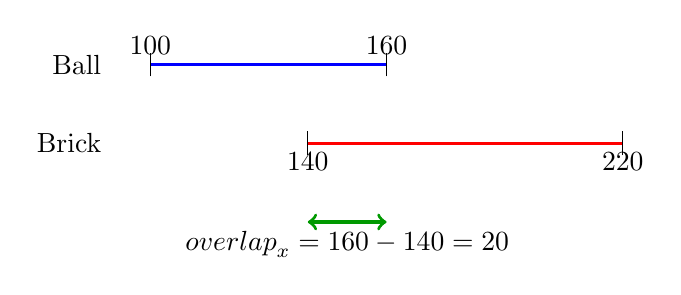
\begin{tikzpicture}[x=0.05cm, y=1cm]
	
	% Ball
	\draw[very thick, blue]
	(100,1) -- (160,1);
	\draw (100,0.85) -- (100,1.15);
	\draw (160,0.85) -- (160,1.15);
	\node[left] at (90,1) {Ball};
	
	% Brick
	\draw[very thick, red]
	(140,0) -- (220,0);
	\draw (140,-0.15) -- (140,0.15);
	\draw (220,-0.15) -- (220,0.15);
	\node[left] at (90,0) {Brick};
	
	% Werte
	\node[above] at (100,1) {100};
	\node[above] at (160,1) {160};
	\node[below] at (140,0) {140};
	\node[below] at (220,0) {220};
	
	% Überlappung
	\draw[very thick, green!60!black, <->]
	(140,-1) -- (160,-1);
	\node[below] at (150,-1) {$\text{overlap}_x = 160 - 140 = 20$};
	
\end{tikzpicture}
\caption{Breakout -- What is $overlap_x$?}
\label{picBreakoutOverlab}
\end{figure}


In the first two lines of the \texttt{bounce()} method, we calculate the horizontal and vertical overlaps. The following \texttt{if} statement uses the criterion described above to determine whether the collision is horizontal or vertical.

In either case, we only need to check whether the ball approaches from the left or right, or from above or below. This would not matter for reversing the direction with \texttt{self.speed.x *= -1}, but we need this information to reposition the ball at the edge of the brick.

In other words, in the example shown in \abbref[vref]{picBreakoutOverlab}, the ball has penetrated \SI{20}{\pixel} into the brick, conveniently ignoring all the laws of physics. In reality, however, it would have stopped at the brick's left edge. We therefore need to move the ball back so that its right edge is aligned with the brick's left edge.


\lstsource{SRC/02 Examples/04 Breakout/v04/breakout.py}{101}{115}{python}{Breakout (\reqref{reqBreakoutCollision}) -- \texttt{Ball.bounce()}}{srcV04ballBounce}

\begin{figure}[htbp]
\centering
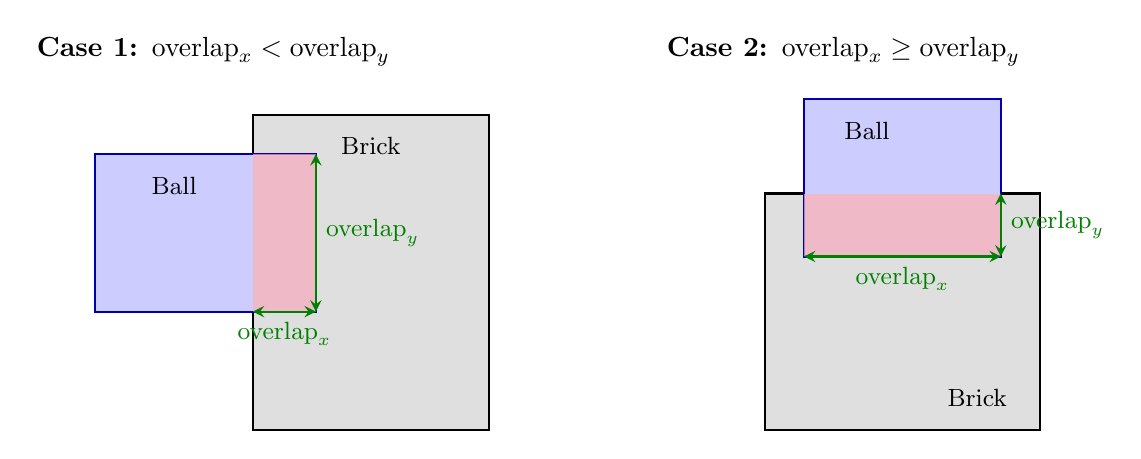
\begin{tikzpicture}[
	scale=1,
	font=\small,
	brick/.style={
		draw=black,
		fill=gray!25,
		thick
	},
	ball/.style={
		draw=blue!70!black,
		fill=blue!20,
		thick
	},
	arrow/.style={
		->,
		>=stealth,
		thick,
		red!70!black
	},
	measure/.style={
		<->,
		>=stealth,
		thick,
		green!50!black
	}
	]
	
	% ============================================================
	% Fall 1: overlap_x < overlap_y
	% ============================================================
	
	\node[font=\bfseries] at (2.5,4.8)
	{Case 1: $\mathrm{overlap}_x < \mathrm{overlap}_y$};
	
	% Brick
	\draw[brick] (3,0) rectangle (6,4);
	\node at (4.5,3.6) {Brick};
	
	% Ball / self.rect
	\draw[ball] (1,1.5) rectangle (3.8,3.5);
	\node at (2.0,3.1) {Ball};
	
	% overlap region
	\fill[red!30,opacity=0.7]
	(3,1.5) rectangle (3.8,3.5);
	
	% overlap_x measurement
	\draw[measure]
	(3,1.5) -- node[below] {$\mathrm{overlap}_x$} (3.8,1.5);
	
	% overlap_y measurement
	\draw[measure]
	(3.8,1.5) -- node[right] {$\mathrm{overlap}_y$} (3.8,3.5);
	
	
	% ============================================================
	% Fall 2: overlap_y <= overlap_x
	% ============================================================
	
	\begin{scope}[xshift=8cm]
		
		\node[font=\bfseries] at (2.5,4.8)
		{Case 2: $\mathrm{overlap}_x \geq \mathrm{overlap}_y$};
		
		% Brick
		\draw[brick] (1.5,0) rectangle (5,3.0);
		\node at (4.2,0.4) {Brick};
		
		% Ball
		\draw[ball] (2,2.2) rectangle (4.5,4.2);
		\node at (2.8,3.8) {Ball};
		
		% overlap region
		\fill[red!30,opacity=0.7]
		(2,2.2) rectangle (4.5,3);
		
		% overlap_x measurement
		\draw[measure]
		(2,2.2) -- node[below] {$\mathrm{overlap}_x$} (4.5,2.2);
		
		% overlap_y measurement
		\draw[measure]
		(4.5,2.2) -- node[right] {$\mathrm{overlap}_y$} (4.5,3);
	\end{scope}
	
\end{tikzpicture}
\caption{Breakout -- Determining the Bounce Direction Based on Rectangle Overlaps}
\label{picBreakoutBounce}
\end{figure}


All that remains is to make the necessary changes to \texttt{Game.update()}. Once the ball has calculated its new position, we identify all bricks that collide with it. There can actually be more than one. Imagine, for example, the ball approaching from below and hitting two bricks simultaneously.

Next, for each colliding brick, we calculate the ball's bounce as described above and notify the brick that it has been hit.

\begin{hintbox}[Why ... ?]
	Why didn't I simply pass \true\ as an argument in \zeiref{breakout0402} to remove the brick immediately?
\end{hintbox}


\lstsource{SRC/02 Examples/04 Breakout/v04/breakout.py}{163}{172}{python}{Breakout (\reqref{reqBreakoutCollision}) -- \texttt{Game.update()}}{srcV04GameUpdate}

\myebild{breakout05}{0.25}{Breakout -- bricks are destroyed and points calculated}{picBreakout05}

Now start the game and let it run after pressing \keys{SPACE}. The bricks should gradually disappear as the ball collides with them, and the points earned should be displayed in the console (see \abbref[vref]{picBreakout05}).

\newpage
%%%%%%%%%%%%%%%%%%%%%%%%%%%%%%%%%%%%%%%%%%%%%%%%%%%%%%%%%%%%%%%%%%%%%
\subsection{\Reqref{reqBreakoutStatus}: Status Bar}

\begin{diskbox}
	\url{https://github.com/adamsralf/pygame_book/tree/main/src/02%20Examples/04%20Breakout/v05}
\end{diskbox}

\br{Status Bar}{reqBreakoutStatus}
The status bar should display:
\begin{enumerate}
	\item the current score,
	\item the number of balls remaining, and
	\item the current game level.
\end{enumerate}
\er

The number of remaining balls and the game level have not yet been given any actual functionality, but we can already include them in the status display.

First, let's define some global variables in \texttt{config.py}.

\lstsource{SRC/02 Examples/04 Breakout/v05/config.py}{17}{22}{python}{Breakout (\reqref{reqBreakoutStatus}) -- \texttt{config.py} with score and level}{srcV05Config}

How should we implement the status bar? On the left, I want to display the number of remaining balls using smaller versions of the ball itself. This is more visually appealing than a simple text display. The score will be shown in the center, and the current level on the right.

I want to avoid re-rendering the status bar's \texttt{Surface} object every frame, even though its content changes only rarely.

\begin{hintbox}[Human Perception vs. Computer Work]
	From a human perspective, the score changes quite frequently. From the computer's perspective, however, it changes only rarely. If the score changes two or three times per second, this means that at \SI{60}{FPS}, it remains unchanged for~57 or~58 frames. Rendering the status bar every frame would therefore result in~57 or~58 completely unnecessary graphics operations.
\end{hintbox}

For this reason, I want to re-render the status bar only when at least one of the three values has changed. Let's implement this now.

First, the constructor creates a \texttt{Surface} object with the same width as the screen and the height specified in \texttt{config.py}. The status information will be rendered onto this \texttt{Surface} object whenever an update is necessary. Next, the ball image is loaded and scaled down to a suitable size.

The attributes \texttt{points}, \texttt{level}, and \texttt{balls} are used to store the values from the last rendering. These three values will later be compared with the current values in \texttt{config.py} to determine whether the status bar needs to be re-rendered.

\lstsource{SRC/02 Examples/04 Breakout/v05/breakout.py}{117}{127}{python}{Breakout (\reqref{reqBreakoutStatus}) -- \texttt{Status.\_\_init\_\_()}}{srcV05StatusInit}

In \texttt{update()}, we check whether at least one of the three values has changed since the last call. If so, the \texttt{Status} class stores the new values and calls \texttt{render()}.

\lstsource{SRC/02 Examples/04 Breakout/v05/breakout.py}{129}{134}{python}{Breakout (\reqref{reqBreakoutStatus}) -- \texttt{Status.update()}}{srcV05StatusUpdate}

\begin{wrapfigure}[12]{r}{7.0cm}%
	\begin{center}%
		\vspace{-6ex}%
		\myfigure{breakout06}{0.25}{Breakout -- status line}{picBreakout06}%
	\end{center}%
\end{wrapfigure}%
The main work is done in \texttt{render()}. First, the status bar is cleared and a suitable font is created. 

Next, the balls are displayed. To do this, the text \verb=Balls:= is rendered and right-aligned. Then, in the \forSchleife, the small balls are vertically centered and displayed next to each other with a spacing of \SI{5}{\pixel}.

The score is then placed in the center of the status bar. For this, the score is rendered as plain text and displayed. Finally, the level information is displayed right-aligned.

\newpage
\lstsource{SRC/02 Examples/04 Breakout/v05/breakout.py}{136}{161}{python}{Breakout (\reqref{reqBreakoutStatus}) -- \texttt{Status.render()}}{srcV05StatusRender}

We have to integrate the class into the game at the usual places. In the \texttt{Game} constructor, a suitable \texttt{GroupSingle} object is created (see \zeiref{breakout0501}). 

\lstsource{SRC/02 Examples/04 Breakout/v05/breakout.py}{178}{179}{python}{Breakout (\reqref{reqBreakoutStatus}) -- \texttt{Game.\_\_init\_\_()}}{srcV05GameInit}

In \zeiref{breakout0502} of \texttt{update()}, the \texttt{Status} object's \texttt{update()} method is called and all that remains is to call \texttt{draw()} in \zeiref{breakout0503} of the \texttt{Game.draw()} method. The temporary console output of the score can now be removed.


\lstsource{SRC/02 Examples/04 Breakout/v05/breakout.py}{219}{220}{python}{Breakout (\reqref{reqBreakoutStatus}) -- \texttt{Game.update()}}{srcV05GameUpdate}

\lstsource{SRC/02 Examples/04 Breakout/v05/breakout.py}{222}{228}{python}{Breakout (\reqref{reqBreakoutStatus}) -- \texttt{Game.draw()}}{srcV05GameDraw}

%\myebild{breakout06}{0.25}{Breakout -- status line}{picBreakout06}

%\newpage
%%%%%%%%%%%%%%%%%%%%%%%%%%%%%%%%%%%%%%%%%%%%%%%%%%%%%%%%%%%%%%%%%%%%%
\subsection{\Reqref{reqBreakoutPaddleBounce}: Ball Bounces off the Paddle}

\begin{diskbox}
	\url{https://github.com/adamsralf/pygame_book/tree/main/src/02%20Examples/04%20Breakout/v06}
\end{diskbox}

\br{Ball Bounces off the Paddle}{reqBreakoutPaddleBounce}
	When the ball hits the central area of the paddle, it bounces back. The farther away from the center the ball hits, the faster and at a steeper angle it is reflected.
\er

The basic idea behind this requirement is to make the game a little more interesting. The closer to the center of the paddle the player hits the ball, the more control they have over its movement.

Since the ball contains a reference to the paddle, we can easily check for a collision between the ball and the paddle directly within the \texttt{Ball} class.

The first two checks in lines~\ref{breakout0603} and~\ref{breakout0604} determine whether any further calculations are necessary, saving processing time. If the vertical velocity is less than~0, the ball is moving upward, so a collision with the paddle cannot have occurred. The second check determines whether the downward-moving ball has collided with the paddle.

Only then does it make sense to calculate the new angle and speed. Before doing so, however, the bottom edge of the ball is corrected in \zeiref{breakout0601}, as the ball may already have penetrated the paddle by a few pixels.

Next, the relative offset is calculated (see \abbref[vref]{picBreakoutBouncePaddle}). This is one of the most important calculations in the method. We want to determine \emph{where the ball hits the paddle}, not in absolute coordinates but relative to the paddle's center: how far to the left, exactly in the middle, or how far to the right.


\begin{figure}
	\begin{center}
	\begin{tikzpicture}[
		>=Stealth,
		font=\small,
		ball/.style={
			circle,
			draw=black!70,
			fill=red!65,
			minimum size=5mm,
			inner sep=0pt
		},
		trajectory/.style={
			->,
			very thick,
			blue!75!black
		}
		]
		% Paddle
		\def\barwidth{10}
		\def\barheight{0.35}
		
		\filldraw[fill=gray!25, draw=black!70, rounded corners=2pt]
		(-5,-0.35) rectangle (5,0);
		
		\node[below=5mm] at (0,-0.15) {Paddle};
		
		% Impact positions and outgoing directions
		\foreach \x/\angle/\off/\velocity in {
			-4.5/-60/-1.0/875,
			-2.25/-30/-0.5/687.5,
			0/0/0.0/500,
			2.25/30/+0.5/687.5,
			4.5/60/+1.0/875
		} {
			% Ball at impact
			\node[ball] at (\x,0.25) {};
			
			% Outgoing trajectory (0 degrees means straight up)
			\draw[trajectory]
			(\x,0.25) --
			++({90-\angle}:2.3);
			
			% Offset labels
			\node[below=10mm, align=center] at (\x,-.30)
			{\texttt{\off}};
		}
		
		% Center line
		\draw[densely dashed, gray]
		(0,-0.6) -- (0,3.4);
		
		% Additional labels
		\node[above] at (0,3.4) {Center};
		\node[below=18mm] at (0,0)
		{\texttt{offset}};
		
	\end{tikzpicture}
	\caption{Breakout -- Ball Bounce Behavior on the Paddle}
	\label{picBreakoutBouncePaddle}
	\end{center}
\end{figure}


First, we calculate the horizontal distance between the center of the ball and the center of the paddle:
\[
	d = x_{\text{ball}} - x_{\text{bar}}
\]

If the ball hits the paddle exactly in the middle, this difference is zero. If it hits on the left, the difference is negative, and if it hits on the right, the difference is positive.

Next, we divide this distance by half the width of the paddle. This is called \emph{normalization}. It gives us a value between $-1$ and $+1$, provided that the center of the ball is within the horizontal boundaries of the paddle.

The resulting value is called \texttt{offset}:

\begin{center}
	\begin{tabular}{rl}
		\toprule
		\texttt{offset} & Impact position \\
		\midrule
		$-1.0$ & Far left \\
		$-0.5$ & Halfway between the left edge and the center \\
		$0.0$  & Exactly in the center \\
		$+0.5$ & Halfway between the center and the right edge \\
		$+1.0$ & Far right \\
		\bottomrule
	\end{tabular}
\end{center}

For example, suppose the paddle is \SI{200}{\pixel} wide and its center is at $x=300$. The ball hits the paddle at $x=250$.
\[
	\text{offset} = \frac{250-300}{200/2} = -0.5
\]

The ball has therefore hit halfway between the center and the left edge of the paddle.


\zeiref{breakout0605} ensures that the offset always stays between $-1$ and $+1$. But why is this necessary? Remember that we detect collisions using rectangles. Two rectangles can overlap even if the center of the ball is already outside the horizontal boundaries of the paddle. This could result in offset values such as $-1.1$ or $+1.2$.\pygindex{math!clamp()}\randnotiz{clamp()}

The offset is then used to determine the speed in \zeiref{breakout0602}. To do this, we calculate how fast the ball should move after the bounce.

The basic speed is \SI{500}{\pixel/\second}. However, we want the ball to move faster when it hits the paddle near one of its edges. To achieve this, we use the absolute value of the offset, calculated with \texttt{abs()}. After all, it should not matter whether the ball hits the left or the right side.

The formula is:
\[
	v = 500 \cdot (1 + 0.75 \cdot |\text{offset}|)
\]

If the ball hits exactly in the center, the offset is zero:
\[
	v = 500 \cdot (1 + 0 \cdot 0.75) = \SI{500}{\pxsec}
\]

If the ball hits at the very edge, the absolute value of the offset is one:
\[
	v = 500 \cdot (1 + 1 \cdot 0.75) = \SI{875}{\pxsec}
\]

So a ball hitting the edge moves \SI{75}{\percent} faster than a ball hitting the center. The following table shows some examples:

\begin{center}
	\begin{tabular}{rr}
		\toprule
		offset & speed (px/s) \\
		\midrule
		$-1.0$ & 875.0 \\
		$-0.5$ & 687.5 \\
		$0.0$  & 500.0 \\
		$+0.5$ & 687.5 \\
		$+1.0$ & 875.0 \\
		\bottomrule
	\end{tabular}
\end{center}

Notice that the speed increases symmetrically towards both edges of the paddle.


Next, we determine in \zeiref{breakout0606} the direction in which the ball should bounce. The maximum bounce angle is $60^\circ$, measured from the vertical direction. This means that a ball hitting the center of the paddle moves straight upwards, while a ball hitting near an edge moves diagonally. The angle is calculated as follows:
\[
	\alpha = 60^\circ \cdot \text{offset}
\]

Here are a few examples:
\begin{center}
	\begin{tabular}{rr}
		\toprule
		offset & Bounce angle \\
		\midrule
		$-1.0$ & $-60^\circ$ \\
		$-0.5$ & $-30^\circ$ \\
		$0.0$  & $0^\circ$ \\
		$+0.5$ & $+30^\circ$ \\
		$+1.0$ & $+60^\circ$ \\
		\bottomrule
	\end{tabular}
\end{center}

A negative angle means that the ball moves to the left, while a positive angle means that it moves to the right. There is one small problem, though: Python's trigonometric functions do not use degrees. They expect angles in \emph{radians}. Fortunately, \texttt{math.radians()} takes care of the conversion for us.

Finally, we need to convert the calculated speed and angle into a velocity vector. A~velocity vector describes both how fast an object moves and in which direction it travels. In our case, it consists of two components:

\begin{itemize}
	\item \texttt{speedxy.x}: the horizontal velocity,
	\item \texttt{speedxy.y}: the vertical velocity.
\end{itemize}

Since our angle is measured from the vertical direction, we use the sine function for the horizontal component and the cosine function for the vertical component:
\begin{align}
	v_x & = v \cdot \sin(\alpha) \nonumber\\
	v_y & = -v \cdot \cos(\alpha) \nonumber
\end{align}

Why the minus sign in the second formula? Remember that in Pygame, the positive y-axis points downwards. Since the ball should bounce upwards, its vertical velocity must be negative.

Let's look at an example. Suppose the ball hits the paddle with an offset of $+0.5$. We already know that this gives us:
\[
	\alpha = 30^\circ
\]

and
\[
	v = \SI{687.5}{\pxsec}
\]

The horizontal and vertical components become:
\begin{align}
	v_x & = 687.5 \cdot \sin(30^\circ) \approx \SI{343.75}{\pxsec}\nonumber\\
	v_y & = -687.5 \cdot \cos(30^\circ) \approx \SI{-595.39}{\pxsec}\nonumber
\end{align}

The ball therefore moves to the right and upwards at the same time. Notice that the overall speed is still \SI{687.5}{\pxsec}. We have simply split it into two components.


\begin{hintbox}[Speed vs. Horizontal and Vertical Velocity]
	The \emph{speed} tells us how fast an object is moving, regardless of its direction. The horizontal and vertical velocities, on the other hand, describe how fast the object moves along the x-axis and y-axis.

	For example, a ball moving diagonally has both a horizontal velocity $v_x$ and a vertical velocity $v_y$. Together, these two components form the \emph{velocity vector}, which describes both the speed and direction of movement (see \abbref[vref]{figVelocity}).

	The actual speed is the length (or magnitude) of this vector and can be calculated using the Pythagorean theorem:
 	\[
 		v = \sqrt{v_x^2 + v_y^2}
 	\]

	For example, if a ball moves at \SI{300}{\pxsec} horizontally and \SI{400}{\pxsec} vertically, its actual speed is \SI{500}{\pxsec}---not \SI{700}{\pxsec}!

	In Pygame, this calculation is particularly easy when using \texttt{pygame.Vector2}: simply call \texttt{self.speed.length()}\pygindex{math!Vector2!length()} to get the actual speed.
\end{hintbox}

\begin{figure}[h]
	\centering
	
	% Farben an den Buchstil anpassbar
	\definecolor{axiscol}{RGB}{120,120,120}
	\definecolor{vxcol}{RGB}{52,152,219}   % blau
	\definecolor{vycol}{RGB}{46,204,113}   % grün
	\definecolor{vcol}{RGB}{231,126,35}    % orange
	\definecolor{pointcol}{RGB}{52,73,94}  % dunkelgrau/blau
	
	\begin{tikzpicture}[>=Stealth, line width=1pt, scale=0.9]
		% Axes
		\draw[->, axiscol] (0,0) -- (5.5,0) node[below, black] {$x$};
		\draw[->, axiscol] (0,0) -- (0,4.5) node[left, black] {$y$};
		
		% Points
		\coordinate (O) at (0,0);
		\coordinate (A) at (3,0);
		\coordinate (B) at (3,4);
		
		% Velocity components
		\draw[->, very thick, vxcol] (O) -- (A)
		node[midway, below, black] {$v_x=\SI{300}{\pxsec}$};
		
		\draw[->, very thick, vycol] (O) -- (0,4)
		node[midway, above, sloped, , pos=0.5, black] {$v_y=\SI{400}{\pxsec}$};
		
		% Resulting velocity
		\draw[->, ultra thick, vcol] (O) -- (B)
		node[midway, above left, sloped, pos=0.8, black] {$v=\SI{500}{\pxsec}$};
		
		% Dashed helper lines
		\draw[dashed, axiscol] (B) -- (0,4);
		\draw[dashed, axiscol] (B) -- (3,0);
		
		% Right angle marker
		\draw[axiscol] (2.6,0) -- (2.6,0.4) -- (3,0.4);
		
		% Labels
		\fill[pointcol] (O) circle (1.2pt) node[below left, black] {start};
		\fill[pointcol] (B) circle (1.2pt) node[above right, black] {ball};
		
	\end{tikzpicture}
	\caption{The horizontal and vertical velocities form a velocity vector.}
	\label{figVelocity}
\end{figure}

You might wonder why we go through all this trouble instead of simply reversing the vertical velocity when the ball hits the paddle. A physically correct bounce from a stationary horizontal paddle would normally reverse the vertical velocity while leaving the horizontal velocity unchanged. For a game like Breakout, however, this would not be particularly exciting. The player would have very little control over the direction of the ball.

Our approach is different:
\begin{itemize}
	\item Hitting the left side sends the ball to the left.
	\item Hitting the center sends the ball straight upwards.
	\item Hitting the right side sends the ball to the right.
	\item Hitting closer to an edge also increases the ball's speed.
\end{itemize}

This gives the player much more control and makes the game more interesting.

\begin{warningbox}
	Our collision detection uses the rectangles of the ball and the paddle. Therefore, a collision can also be detected when the ball touches the paddle from the side.
	
	As long as the ball is moving downwards, our method will treat this as a bounce from the top. For a simple Breakout game, this is often good enough. A more accurate collision system would also check which side of the paddle was hit.
\end{warningbox}

So, in just a few lines of code, \texttt{bounce\_paddle()} performs three important tasks: it detects a collision, corrects the ball's position, and calculates a new trajectory that the player can influence.

\lstsource{SRC/02 Examples/04 Breakout/v06/breakout.py}{101}{114}{python}{Breakout (\reqref{reqBreakoutPaddleBounce}) -- \texttt{Ball.bounce\_paddle()}}{srcV06BallBouncePaddle}

\newpage
%%%%%%%%%%%%%%%%%%%%%%%%%%%%%%%%%%%%%%%%%%%%%%%%%%%%%%%%%%%%%%%%%%%%%
\subsection{\Reqref{reqBreakoutAutopilot}: Autopilot}

\begin{diskbox}
	\url{https://github.com/adamsralf/pygame_book/tree/main/src/02%20Examples/04%20Breakout/v07}
\end{diskbox}

\br{Autopilot}{reqBreakoutAutopilot}
\begin{enumerate}
	\item Pressing \keys{F2} should toggle the autopilot on and off.
	\item When the autopilot is enabled, the background color should change to dark green.
\end{enumerate}
\er

The autopilot is not primarily intended for bored players, but rather as a useful testing tool. Later, I can use it to test level transitions and increasing difficulty. I'll start by defining the \texttt{AUTOPILOT} flag in \texttt{config.py}.

\lstsource{SRC/02 Examples/04 Breakout/v07/config.py}{22}{26}{python}{Breakout (\reqref{reqBreakoutAutopilot}) -- \texttt{AUTOPILOT}}{srcV07Config}

In \texttt{watch\_for\_events()}, we now check whether the autopilot is disabled, because only then are the arrow key events forwarded to the paddle (see \zeiref{breakout0702} and~\zeiref{breakout0703}). Starting at \zeiref{breakout0704}, pressing \keys{F2} toggles the flag.

\lstsource{SRC/02 Examples/04 Breakout/v07/breakout.py}{212}{229}{python}{Breakout (\reqref{reqBreakoutAutopilot}) -- \texttt{Game.watch\_for\_events()}}{srcV07WatchForEvents}

In \texttt{update()}, we now implement a simple autopilot logic. The basic idea is:
\begin{itemize}
	\item If the right edge of the ball is to the right of the paddle's left edge, the paddle must move to the left.
	\item If the left edge of the ball is to the left of the paddle's right edge, the paddle must move to the right.
	\item Otherwise, the paddle can remain stationary.
\end{itemize}

\lstsource{SRC/02 Examples/04 Breakout/v07/breakout.py}{231}{250}{python}{Breakout (\reqref{reqBreakoutAutopilot}) -- \texttt{Game.update()}}{srcV07Update}

All that remains is to set the background color. This is also done simply by checking the \texttt{AUTOPILOT} flag in \texttt{draw()}.

\lstsource{SRC/02 Examples/04 Breakout/v07/breakout.py}{252}{261}{python}{Breakout (\reqref{reqBreakoutAutopilot}) -- \texttt{Game.draw()}}{srcV07Draw}

\newpage
%%%%%%%%%%%%%%%%%%%%%%%%%%%%%%%%%%%%%%%%%%%%%%%%%%%%%%%%%%%%%%%%%%%%%
\subsection{\Reqref{reqBreakoutGameEnd}: Game Over}

\begin{diskbox}
	\url{https://github.com/adamsralf/pygame_book/tree/main/src/02%20Examples/04%20Breakout/v08}
\end{diskbox}

\br{Game Over}{reqBreakoutGameEnd}
\begin{enumerate}
	\item Whenever the ball touches the bottom edge of the playing field, the player loses a ball.
	\item When the player loses a ball, the paddle returns to the center and starts again with a new ball.
\end{enumerate}
\er

We now need to reset both the paddle and the ball, as they should start again from the center. To achieve this, I'll add a \texttt{reset()} method to the paddle.

\lstsource{SRC/02 Examples/04 Breakout/v08/breakout.py}{100}{103}{python}{Breakout (\reqref{reqBreakoutGameEnd}) -- \texttt{Ball.reset()}}{srcV08BallReset()}

This method can now also be used in the constructor.

\lstsource{SRC/02 Examples/04 Breakout/v08/breakout.py}{62}{71}{python}{Breakout (\reqref{reqBreakoutGameEnd}) -- Calling \texttt{reset()} in \texttt{Ball.\_\_init\_\_()}}{srcV08BallInit()}

The \texttt{Paddle} class is extended in exactly the same way:

\lstsource{SRC/02 Examples/04 Breakout/v08/breakout.py}{56}{59}{python}{Breakout (\reqref{reqBreakoutGameEnd}) -- \texttt{Paddle.reset()}}{srcV08PaddleReset()}

\lstsource{SRC/02 Examples/04 Breakout/v08/breakout.py}{34}{41}{python}{Breakout (\reqref{reqBreakoutGameEnd}) -- Calling \texttt{reset()} in \texttt{Paddle.\_\_init\_\_()}}{srcV08PaddleInit()}

However, we also need a helper method in the \texttt{Ball} class to determine whether the ball has been lost. I'll give it the descriptive name \texttt{is\_lost()}.

\lstsource{SRC/02 Examples/04 Breakout/v08/breakout.py}{136}{137}{python}{Breakout (\reqref{reqBreakoutGameEnd}) -- \texttt{Ball.is\_lost()}}{srcV08PaddleIsLost()}

\begin{wrapfigure}[13]{r}{7.0cm}%
	\begin{center}%
		\vspace{-6ex}%
		\myfigure{breakout07}{0.25}{Breakout -- after losing a ball}{picBreakout07}%
	\end{center}%
\end{wrapfigure}%
With these preparations in place, the rest is straightforward. Starting at \zeiref{breakout0801}, the \texttt{Game.update()} method is extended with the corresponding logic.

First, we check whether the ball has been lost. If so, the number of remaining balls is reduced by~1. Next, we check whether any balls are left. If \emph{not}, the flag controlling the main game loop is set to \false, which terminates the program. If \emph{yes}, the positions of the \texttt{Paddle} and \texttt{Ball} are reset, and the game continues.

Everything else -- such as updating the number of remaining balls in the status bar -- happens automatically.

\lstsource{SRC/02 Examples/04 Breakout/v08/breakout.py}{237}{263}{python}{Breakout (\reqref{reqBreakoutGameEnd}) -- \texttt{Game.update()}}{srcV08PaddleUpdate()}

In \abbref[vref]{picBreakout07}, you can see what the status bar, ball, and paddle look like after a ball has been lost.

%%%%%%%%%%%%%%%%%%%%%%%%%%%%%%%%%%%%%%%%%%%%%%%%%%%%%%%%%%%%%%%%%%%%%
\subsection{\Reqref{reqBreakoutLevel}: Increasing Difficulty}

\begin{diskbox}
	\url{https://github.com/adamsralf/pygame_book/tree/main/src/02%20Examples/04%20Breakout/v09}
\end{diskbox}

\br{Increasing Difficulty}{reqBreakoutLevel}
\begin{enumerate}
	\item The game starts with three rows of bricks.
	\item When all bricks have been destroyed, the game restarts with one additional row.
	\item A maximum of 9~rows is displayed.
	\item Each time the game restarts, the level counter is increased by~1.
	\item With each new level, the proportion of bricks that require two hits to break increases.
	\item At each level transition, the player receives one additional ball.
\end{enumerate}
\er

As a first step, let's modify the \texttt{Brick} class so that it can display not just one image, but a second one if necessary.

In \zeiref{breakout1001}, a list is created that can hold multiple images if necessary. The following line determines whether we need one or two images for the brick -- in other words, whether the brick is cracked before it is completely destroyed.

To do this, \texttt{random.random()}\index{random!random()}\randnotiz{random()} generates a uniformly distributed random number from the interval~$[0, 1)$. The following condition only makes sense once you understand the idea behind it.

I want the level number (\texttt{cfg.LEVEL}) to determine the probability that a brick needs two hits to break. Each level should increase this probability by \SI{10}{\percent} points, as shown in \tabref{tabLevelProb}. To convert \texttt{LEVEL} into a probability, we therefore need to divide it by~10: \texttt{cfg.LEVEL / 10}.

But what happens when the level number exceeds~10? Since the probability should not exceed \SI{100}{\percent}, we limit the level number used in the calculation to~10. This gives us \texttt{min(cfg.LEVEL, 10) / 10}.

\begin{longtable}{rr@{ $\widehat{=}$ }r}
	\caption{Level $\rightarrow$ Probability}\label{tabLevelProb} \\
	% Definition des Tabellenkopfes auf der ersten Seite
	\toprule
	Level  & Probability & \%\\
	\midrule
	\endfirsthead % Erster Kopf zu Ende
	
	% Definition des Tabellenkopfes auf den folgenden Seiten
	\caption{Level $\rightarrow$ Probability (continued)}\\
	\toprule
	Level  & Probability & \%\\
	\midrule
	\endhead % Zweiter Kopf ist zu Ende
	
	\midrule
	\multicolumn{3}{r}{\emph{continued on next page}} \\
	\endfoot
	
	\bottomrule
	\endlastfoot
	% Ab hier kommt der Inhalt der Tabelle
	1 &  $0.1$ & $\SI{10}{\%}$\\ 
	2 &  $0.2$ & $\SI{20}{\%}$\\ 
	\multicolumn{3}{c}{$\cdots$}\\
	8 &  $0.8$ & $\SI{80}{\%}$\\ 
	9 &  $0.9$ & $\SI{90}{\%}$\\ 
	10 &  $1.0$ & $\SI{100}{\%}$\\ 
	$>10$ &  $1.0$ & $\SI{100}{\%}$
\end{longtable} 

If a random number between~0 and~1 is smaller than the probability defined by \texttt{cfg.LEVEL}, \texttt{image\_count} is set to~2; otherwise, it is set to~1. In the following \forSchleife, the images are loaded, and \texttt{self.image} is assigned the appropriate image using \texttt{imageindex}.

\lstsource{SRC/02 Examples/04 Breakout/v09/breakout.py}{11}{28}{python}{Breakout (\reqref{reqBreakoutLevel}) -- \texttt{Brick.\_\_init\_\_()}}{srcV09BBrickInit()}

All that remains is to adjust how a brick reacts when it is hit. In \texttt{hit()}, we check whether the current \texttt{imageindex} has already reached the end of the list of available images. This is a bit of overkill, since we have at most~2 images. If not, \texttt{imageindex} is increased by~1 -- from~0 to~1 -- and \texttt{self.image} is assigned the other image.

However, if \texttt{imageindex} has already reached the end of the list -- meaning it has the value~1 -- the score is increased and the brick is removed, just as before. Verify for yourself that this logic also works for bricks that have only one image and therefore break immediately.

\lstsource{SRC/02 Examples/04 Breakout/v09/breakout.py}{35}{41}{python}{Breakout (\reqref{reqBreakoutLevel}) -- \texttt{Brick.hit()}}{srcV09BBrickHit()}

Since the bricks need to be recreated at each level transition, I have moved their creation into a separate method and called it from \texttt{\_\_init\_\_()} (\zeiref{breakout0902}).

\lstsource{SRC/02 Examples/04 Breakout/v09/breakout.py}{198}{213}{python}{Breakout (\reqref{reqBreakoutLevel}) -- \texttt{Game.\_\_init\_\_()}}{srcV09BGameInit()}

The functionality of \texttt{create\_bricks()} has already been explained above. It contains nothing new, apart from clearing the \texttt{sprite.Group} as a precaution using \texttt{empty()}\pygindex{sprite!Group!empty()}\randnotiz{empty()}.

\lstsource{SRC/02 Examples/04 Breakout/v09/breakout.py}{215}{220}{python}{Breakout (\reqref{reqBreakoutLevel}) -- \texttt{Game.create\_bricks()}}{srcV09BGameCreateBrick()}

The game has now reached a point where it can actually be played with all the essential Breakout mechanics in place. What follows are mainly visual improvements and a few minor features.

\newpage
%%%%%%%%%%%%%%%%%%%%%%%%%%%%%%%%%%%%%%%%%%%%%%%%%%%%%%%%%%%%%%%%%%%%%
\subsection{\Reqref{reqBreakoutScenes}: Scenes}

\begin{diskbox}
	\url{https://github.com/adamsralf/pygame_book/tree/main/src/02%20Examples/04%20Breakout/v10}
\end{diskbox}

\begin{hintbox}
	Unlike in the previous chapters, I will not document the individual steps of restructuring the code here. I tried this in an earlier version of the text, but the result turned out to be rather confusing. Instead, I will present and explain the final versions of the source files.
\end{hintbox}

\begin{figure}[htb]
	\centering
	%	\vspace{-1.0em}
	\definecolor{pygblue}{RGB}{220,235,250}
	\definecolor{hintgreen}{RGB}{225,245,230}
	\definecolor{iconred}{RGB}{150,40,40}
	\begin{tikzpicture}[
		node distance=3mm and 3mm, % (vertikal) and (horizontal)
		n/.style={anchor=west},
		e/.style={draw=black!50, line width=0.4pt},
		folder/.style={
			font=\ttfamily\small,
			draw=black!40,
			rounded corners=2pt,
			inner sep=2pt,
			fill=pygblue,
			align=left,
			text width=35mm,
			draw=none
		},
		dots/.style={
			draw=black!40,
			rounded corners=2pt,
			inner ysep=4pt,
			fill=white,
			align=left,
			text width=35mm
		},
		file/.style={
			font=\ttfamily\small,
			draw=black!30,
			rounded corners=2pt,
			inner sep=2pt,
			fill=hintgreen,
			align=left,
			text width=35mm,
			draw=none
		}
		]
		\pgfmathsetmacro{\row}{7} % mm pro Zeile
		
		\node[folder] (root) {\textcolor{iconred}{\faFolder\ }breakout/};
		\path (root.west) coordinate (L0);
		\coordinate (L1) at ($(L0)+(9mm,0)$);
		\coordinate (L2) at ($(L1)+(9mm,0)$);
		\coordinate (L3) at ($(L2)+(9mm,0)$);
		
		% top level (Ebene 0)
		\node[n, file] at ($(L1 |- root)   + (0mm,-\row mm)$) (main)   {\textcolor{iconred}{\faFile\ }main.py};
		\node[n, file] at ($(L1 |- main)   + (0mm,-\row mm)$) (config) {\textcolor{iconred}{\faFile\ }config.py};
		\node[n, folder] at ($(L1 |- config) + (0mm,-\row mm)$) (assets) {\textcolor{iconred}{\faFolder\ }assets/};
		
		% assets children (Ebene 1)
		\node[n, folder] at ($(L2 |- assets) + (0mm,-\row mm)$) (images) {\textcolor{iconred}{\faFolder\ }images/};
		\node[n, file] at ($(L3 |- images)   + (0mm,-\row mm)$) (imageball)   {\textcolor{iconred}{\faFile\ }ball.png};
		\node[n, file] at ($(L3 |- imageball)   + (0mm,-\row mm)$) (imagebar)   {\textcolor{iconred}{\faFile\ }bar.png};
		\node[n, file] at ($(L3 |- imagebar)   + (0mm,-\row mm)$) (imagebricka)   {\textcolor{iconred}{\faFile\ }brick0000.png};
		\node[n, file] at ($(L3 |- imagebricka)   + (0mm,-\row mm)$) (imagebrickb)   {\textcolor{iconred}{\faFile\ }...};
		\node[n, file] at ($(L3 |- imagebrickb)   + (0mm,-\row mm)$) (imagebrickc)   {\textcolor{iconred}{\faFile\ }brick0901.png};
		
		% next top level (Ebene 0), aligned left
		\node[n, folder] at ($(L1 |- imagebrickc) + (0mm,-\row mm)$) (scenes) {\textcolor{iconred}{\faFolder\ }scenes/};
		
		% scenes children (Ebene 1)
		\node[n, file] at ($(L2 |- scenes) + (0mm,-\row mm)$) (stateinit)  {\textcolor{iconred}{\faFile\ }\_\_init\_\_.py};
		\node[n, file] at ($(L2 |- stateinit) + (0mm,-\row mm)$) (state)  {\textcolor{iconred}{\faFile\ }state.py};
		\node[n, file] at ($(L2 |- state)   + (0mm,-\row mm)$) (gameover)  {\textcolor{iconred}{\faFile\ }gameover.py};
		\node[n, file] at ($(L2 |- gameover)   + (0mm,-\row mm)$) (help) {\textcolor{iconred}{\faFile\ }help.py};
		\node[n, file] at ($(L2 |- help)   + (0mm,-\row mm)$) (pause) {\textcolor{iconred}{\faFile\ }pause.py};
		\node[n, file] at ($(L2 |- pause)   + (0mm,-\row mm)$) (play) {\textcolor{iconred}{\faFile\ }play.py};
		\node[n, file] at ($(L2 |- play)   + (0mm,-\row mm)$) (start) {\textcolor{iconred}{\faFile\ }start.py};
		
		% next top level
		\node[n, folder] at ($(L1 |- start) + (0mm,-\row mm)$) (sprites) {\textcolor{iconred}{\faFolder\ }sprites/};
		
		% sprites children
		\node[n, file] at ($(L2 |- sprites) + (0mm,-\row mm)$) (spriteinit)  {\textcolor{iconred}{\faFile\ }\_\_init\_\_.py};
		\node[n, file] at ($(L2 |- spriteinit)  + (0mm,-\row mm)$) (spriteball) {\textcolor{iconred}{\faFile\ }ball.py};
		\node[n, file] at ($(L2 |- spriteball) + (0mm,-\row mm)$) (spritebrick)  {\textcolor{iconred}{\faFile\ }brick.py};
		\node[n, file] at ($(L2 |- spritebrick) + (0mm,-\row mm)$) (spritepaddle)  {\textcolor{iconred}{\faFile\ }paddle.py};
		\node[n, file] at ($(L2 |- spritepaddle) + (0mm,-\row mm)$) (spritestatus)  {\textcolor{iconred}{\faFile\ }status.py};
		

		% Connect root to each top-level entry
		\draw[e] (root.west) ++(-2mm,0) -- ++(2mm,0); % small stub (optional)
		\foreach \x in {main,config,assets,scenes,sprites} {
			\draw[e] (root.south west) ++(0,-0.5mm) |- (\x.west);
		}
		
		% Level 2: assets children (indented to the right)
		
		\foreach \x in {images} {
			\draw[e] (assets.south west) ++(0,-0.5mm) |- (\x.west);
		}
		
		% Level 3: image children (indented to the right)

		\foreach \x in {imageball, imagebar, imagebricka, imagebrickb, imagebrickc} {
			\draw[e] (images.south west) ++(0,-0.5mm) |- (\x.west);
		}

		% Level 2: scenes children
		
		\foreach \x in {stateinit, state, gameover, help, pause, play, start} {
			\draw[e] (scenes.south west) ++(0,-0.5mm) |- (\x.west);
		}
		
		% Level 2: sprites children
		
		\foreach \x in {spriteinit, spriteball, spritebrick, spritepaddle, spritestatus} {
			\draw[e] (sprites.south west) ++(0,-0.5mm) |- (\x.west);
		}
	
	\end{tikzpicture}
	\caption{Breakout -- directories and files}\label{figBreakoutFiles}
\end{figure}

\br{Scenes}{reqBreakoutScenes}
\begin{enumerate}
	\item When the game starts, the player is welcomed and an introduction is displayed.
	\item Pressing \keys{P} pauses or resumes the game.
	\item Pressing \keys{H} shows or hides the help text.
	\item When all balls have been lost, the game ends and asks the player whether they want to play again.
	\item If the player wants to play again, the game starts completely anew.
	\item If the player does not want to play again, the game says goodbye with a farewell message.
\end{enumerate}
\er

To fulfill \reqref{reqBreakoutScenes}, we need to restructure the internal architecture of the program. I will follow the approach described in \secref[vref]{secStateMachine}.\index{State Machine}\index{Scenes} The project structure will also be reorganized according to \secref[vref]{secProjStruct}. Here is an overview of the necessary steps:

\begin{enumerate}
	\item Rename \texttt{breakout.py} to \texttt{main.py}.
	\item Move the classes \texttt{Ball}, \texttt{Brick}, \texttt{Paddle}, and \texttt{Status} into separate files in the \texttt{sprites} subdirectory.
	\item Create the abstract base class \texttt{State} in \texttt{state.py} within the new \texttt{scenes} subdirectory.
	\item In the same subdirectory, create the files \texttt{gameover.py}, \texttt{help.py}, \texttt{pause.py}, \texttt{start.py}, and \texttt{play.py}, each containing the corresponding implementation of \texttt{State}.
	\item Refactor \texttt{main.py} to use the new architecture.
\end{enumerate}

The resulting project structure is shown in \abbref[vref]{figBreakoutFiles}.

\clearpage

Let's start with \texttt{main.py}. The source code in \srcref{srcV10BreakoutMain} is now nicely organized and, following the \Gls{srp}, focuses exclusively on managing the scenes and the main game loop.

Although it may sound a little repetitive, the code is actually very similar to the implementation presented in \secref[vref]{secStateMachine}. Therefore, most of the explanations from that section also apply here.

The \texttt{Game} class is the central controller of our Breakout game; it manages the game window, the main game loop, and the different game states. Instead of implementing the entire game logic itself, it delegates state-specific tasks to subclasses of the abstract \texttt{State} class.

The most important attribute is \texttt{stack\_state}, a list that stores the currently active states. The methods \texttt{push\_state()}, \texttt{pop\_state()}, and \texttt{replace\_state()} manage this stack. The property \texttt{current\_state} provides access to the state at the top of the stack.

The state machine diagram (\abbref{picBreakoutStateMachine}) illustrates how the game switches between its states. The game begins in \texttt{StartState}, switches to \texttt{PlayState} when the player presses \keys{SPACE}, and enters \texttt{GameOverState} when no balls remain. The \texttt{PauseState} and \texttt{Help\-State} are temporary states that are pushed onto the stack. When they are removed, the previous state automatically becomes active again.

The main game loop in \texttt{run()} repeatedly calls \texttt{watch\_for\_events()}, \texttt{update()}, and \texttt{draw()}. While events and updates are forwarded only to the current state, all states in the stack are drawn in order. This allows temporary overlays, such as the help screen, to appear on top of the game while the underlying game logic remains paused.

This design keeps the \texttt{Game} class relatively simple and separates the management of the game from the implementation of individual game states.

\lstsource{SRC/02 Examples/04 Breakout/v10/main.py}{1}{87}{python}{Breakout (\reqref{reqBreakoutScenes}) -- \texttt{main.py}}{srcV10BreakoutMain}

The classes \texttt{Ball}, \texttt{Brick}, \texttt{Status}, and \texttt{Paddle} have not changed at all, apart from their location in the project structure. Therefore, no further explanation is necessary.

What makes things interesting now are the state classes -- the scenes. The base class \texttt{State} consists almost entirely of abstract methods. Its \texttt{\_\_init\_\_()} method simply stores a reference to the \texttt{Game} object, allowing the scenes to access other components of the game, such as \texttt{self.game.screen}. It also provides two fonts that are used in \texttt{draw\_message()}.

\lstsource{SRC/02 Examples/04 Breakout/v10/scenes/state.py}{8}{99}{python}{Breakout (\reqref{reqBreakoutScenes}) -- \texttt{state.py}}{srcV10BreakoutState}

The classes \texttt{GameOverState} (\srcref{srcV10BreakoutGameover}), \texttt{HelpState} (\srcref{srcV10BreakoutHelp}), and \texttt{PauseState} (\srcref{srcV10BreakoutPause}) are very similar. They handle the keyboard events that trigger a return to the game or the next appropriate state (see \abbref[vref]{picBreakoutStateMachine}) and display predefined messages from \texttt{config.py}.

\lstsource{SRC/02 Examples/04 Breakout/v10/scenes/gameover.py}{7}{20}{python}{Breakout (\reqref{reqBreakoutScenes}) -- \texttt{gameover.py}}{srcV10BreakoutGameover}

\lstsource{SRC/02 Examples/04 Breakout/v10/scenes/help.py}{7}{17}{python}{Breakout (\reqref{reqBreakoutScenes}) -- \texttt{help.py}}{srcV10BreakoutHelp}

\lstsource{SRC/02 Examples/04 Breakout/v10/scenes/pause.py}{7}{20}{python}{Breakout (\reqref{reqBreakoutScenes}) -- \texttt{pause.py}}{srcV10BreakoutPause}

All that remains is the actual gameplay class, \texttt{PlayState}. Don't be intimidated by its length, as most of the code consists of game logic we have already discussed.

\lstsource{SRC/02 Examples/04 Breakout/v10/scenes/play.py}{8}{96}{python}{Breakout (\reqref{reqBreakoutScenes}) -- \texttt{play.py}}{srcV10BreakoutPlay}

\begin{figure}[htb]
	\centering
	\begin{tikzpicture}[
		scale=0.8,
		transform shape,
		>=Latex,
		state/.style={
			rectangle,
			rounded corners,
			draw=blue!65!black,
			thick,
			minimum width=3.6cm,
			minimum height=1cm,
			align=center,
			fill=blue!8
		},
		overlay/.style={
			state,
			draw=teal!70!black,
			fill=teal!10
		},
		final/.style={
			circle,
			draw,
			thick,
			minimum size=0.65cm,
			fill=black
		},
		transition/.style={
			-{Latex[length=2.5mm]},
			thick
		},
		stack/.style={
			transition,
			dashed,
			draw=teal!70!black
		},
		note/.style={
			font=\small,
			align=center,
			fill=white,
			inner sep=2pt
		}
		]
		
		% Main states
		\node[final] (init) at (0,0) {};
		\node[state] (start) at (5,0) {\textbf{StartState}};
		\node[state] (play) at (5,-5) {\textbf{PlayState}};
		\node[state] (over) at (5,-10) {\textbf{GameOverState}};
		\node[final] (end) at (5,-14) {};
		
		% Overlay states
		\node[overlay] (pause) at (13,-2) {\textbf{PauseState}};
		\node[overlay] (help) at (13,-8) {\textbf{HelpState}};
		
		% Initial transition
		\draw[transition] (init) --	node[above] {create game} (start);
		
		% Main game flow
		\draw[transition] (start) -- node[left] {\keys{SPACE}: replace\_state()} (play);
		\draw[transition] (play) --	node[left] {no balls left} (over);
		
		% Restart
		\draw[transition] (over.west) -- ++(-2,0)|- node[pos=0.25, left] {\keys{Y}: start\_new\_game()}	(play.west);
		
		% Game over -> Exit
		\draw[transition] (over) --	node[right] {\keys{N}} (end);
		
		% Play -> Pause	
		\draw[stack] (play.north east) --	node[above, sloped] {\keys{P}: push\_state()} (pause.west);
		
		% Pause -> Play
		\draw[stack] (pause.south) -- ++(0,-1.00) |- node[pos=.1, right] {\keys{P}: pop\_state()}(play.east);
		
		% Play -> Help
		\draw[stack] (play.south east) -- node[below, sloped] {\keys{H}: push\_state()} (help.west);
		
		% Help -> Play
		\draw[stack] (help.north) -- ++(0,1.0) |- node[pos=.1, right] {\keys{H}: pop\_state()}(play.east);
		
		% Global exit note
		\node[note, anchor=west, right=2 of end.east] (endtext) {\keys{ESC}, \keys{Q}, quit: from every state};
		
		\draw[transition, dashed] (endtext.west) -- (end.east);
		
	\end{tikzpicture}
	
	\caption{Breakout -- State machine with temporary
		overlay states}
	\label{picBreakoutStateMachine}
\end{figure}

Give it a try! The game should now respond to game events and the \keys{P} and \keys{H} keys.

\newpage
%%%%%%%%%%%%%%%%%%%%%%%%%%%%%%%%%%%%%%%%%%%%%%%%%%%%%%%%%%%%%%%%%%%%%
\subsection{\Reqref{reqBreakoutTrail}: Trail of the Ball}

\begin{diskbox}
	\url{https://github.com/adamsralf/pygame_book/tree/main/src/02%20Examples/04%20Breakout/v11}
\end{diskbox}

\br{Trail of the Ball}{reqBreakoutTrail}
	The ball leaves a trail of smaller and smaller balls behind it, which gradually fade away. This effect is purely visual and has no influence on the game logic.
\er

The basic idea behind my solution is to create a copy of the ball every \SI{10}{ms} and store it in a separate list. These copies (objects of the \texttt{TrailBall} class) are gradually scaled down using \texttt{pygame.transform.scale\_by()}\pygindex{transform!scale\_by()}, while their transparency is increased using \texttt{pygame.Surface.set\_alpha()}\pygindex{Surface!set\_alpha()}.

Let's take a look at the \texttt{TrailBall} class in \srcref{srcV11BreakoutTrailBall}. First, I define the class attribute \texttt{TRAIL\_DURATION} and set it to \SI{0.4}{\second}. This value determines how long each fading ball remains visible. After some experimenting, I settled on \SI{400}{\milli\second}.

The constructor receives the \texttt{Ball} object so that it can make a copy of its image and position. The lifetime of the new trail ball, stored in \texttt{remaining}, is also initialized with \texttt{TRAIL\_DURATION}.

In the \texttt{update()} method, we first check whether the trail ball has any \emph{lifetime} left -- in other words, whether the \SI{400}{\milli\second} have already passed. If there is still some time left, we subtract the time elapsed since the last call to \texttt{update()} from \texttt{remaining}. Then, we make the image smaller and increase its transparency.

Once the lifetime has run out, the sprite is removed from all sprite groups using \texttt{kill()}\pygindex{sprite!Sprite!kill()}. If no references to the object remain, Python can also remove it from memory.

\lstsource{SRC/02 Examples/04 Breakout/v11/sprites/trailball.py}{9}{25}{python}{Breakout (\reqref{reqBreakoutTrail}) -- \texttt{trailball.py}}{srcV11BreakoutTrailBall}

In the constructor of \texttt{PlayState}, we need to add a few things. First, there is the list \texttt{trail}, which stores all the \texttt{TrailBall} objects. Next, we add two attributes that control when the next \texttt{TrailBall} is created.

Why do we need this kind of control? Without it, a new \texttt{TrailBall} would be created every frame -- that is, FPS times per second. We wouldn't even be able to see most of them!

Feel free to set \texttt{trail\_freq} to~1 and see if you notice any difference.

\lstsource{SRC/02 Examples/04 Breakout/v11/scenes/play.py}{19}{22}{python}{Breakout (\reqref{reqBreakoutTrail}) -- \texttt{PlayState.\_\_init\_\_()}}{srcV11BreakoutPlayInit}

\begin{wrapfigure}[12]{r}{7.0cm}%
	\begin{center}%
		\vspace{-6ex}%
		\myfigure{breakout08}{0.25}{Breakout -- ball with trail}{picBreakout08}%
	\end{center}%
\end{wrapfigure}%
The \texttt{update()} method is now extended with the logic for creating the trail. In \zeiref{breakoutplay1101}, we check whether enough time has passed since the last \texttt{TrailBall} was created. As mentioned before, this prevents us from creating an unnecessarily large number of them.

If \emph{yes}, a new \texttt{TrailBall} object is created and added to the trail, and the time for creating the next \texttt{TrailBall} is calculated.

Finally, all \texttt{TrailBall} objects in the list are updated, causing them to become smaller and more transparent.

That's it! The result is shown in \abbref[vref]{picBreakout08}.

\lstsource{SRC/02 Examples/04 Breakout/v11/scenes/play.py}{60}{66}{python}{Breakout (\reqref{reqBreakoutTrail}) -- \texttt{PlayState.update()}}{srcV11BreakoutPlayUpdate()}

\newpage
%%%%%%%%%%%%%%%%%%%%%%%%%%%%%%%%%%%%%%%%%%%%%%%%%%%%%%%%%%%%%%%%%%%%%
\subsection{\Reqref{reqBreakoutBrickApart}: Brick Breaks Apart}

\begin{diskbox}
	\url{https://github.com/adamsralf/pygame_book/tree/main/src/02%20Examples/04%20Breakout/v12}
\end{diskbox}

\br{Bricks break apart}{reqBreakoutBrickApart}
	When a brick breaks, it should fall apart into individual pieces that tumble downward. As they fall, they gradually fade away.
\er

As with the trail, we'll create a new class for this effect: \texttt{BrickFragment}. Its job is to copy a part of a brick's \texttt{Surface} and let it fall downward with its own velocity and rotation in \texttt{update()}.

The class attribute \texttt{DURATION} works just like in \texttt{TrailBall}, while \texttt{FADE\_DURATION} determines when the fragment starts to fade, measured backward from the end of its lifetime (more on this when we look at \texttt{update()}).

Now let's take a look at the constructor. The first few lines calculate which part of the brick this fragment should represent. For this, we need the values \texttt{col} and \texttt{row}. Using the column number \texttt{col} and the column width \texttt{width}, we can calculate the fragment's left edge, \texttt{left}. Similarly, the row number \texttt{row} and the row height \texttt{height} give us its top edge, \texttt{top}. We can then use \texttt{Surface.subsurface()}\pygindex{Surface!subsurface()}\randnotiz{subsurface()} to cut out the fragment and assign it to \texttt{self.image}.

Next, we initialize the movement and rotation. With \texttt{spin\_direction}, I randomly choose whether the fragment rotates to the left ($-1$) or to the right ($+1$). For \texttt{angular\-\_velocity}, this randomly chosen direction is combined with a random rotation speed between \SI{100}{\degree\per\second} and \SI{240}{\degree\per\second}. Depending on the direction and the random value, each fragment spins faster or slower. This makes the breaking effect look more realistic.

Now, we define \texttt{self.rect} for the \texttt{Sprite} class and set it to the fragment's starting position.

All that remains is the falling velocity, \texttt{velocity}. The random values are chosen so that the fragments spread out to the left and right. Each fragment also gets its own random vertical velocity, which is negative so that the fragment initially moves upwards.

\lstsource{SRC/02 Examples/04 Breakout/v12/sprites/brickfragment.py}{11}{28}{python}{Breakout (\reqref{reqBreakoutBrickApart}) -- \texttt{BrickFragment.\_\_init\_\_()}}{srcV12BreakoutBrickFragmentInit}

\begin{wrapfigure}[12]{r}{7.0cm}%
	\begin{center}%
		\vspace{-6ex}%
		\myfigure{breakout09}{0.25}{Breakout -- bricks break apart}{picBreakout09}%
	\end{center}%
\end{wrapfigure}%
In the first line of \texttt{update()}, the fragment's remaining lifetime is reduced. The next two lines use a somewhat arbitrary gravity value to accelerate the fragment as it falls.

The following four lines handle the rotation. First, I store the current center position of the fragment. I need this because rotating an image can change its position. After the rotation, I use the saved center to put the fragment back in the right place. In between, the new angle is calculated and kept within the range from~$0$ to~$360$ using the modulo operator.

The final part of \texttt{update()} deals with removing the fragment and making it fade away. First, we check whether its lifetime has expired. If \emph{yes}, the \texttt{Sprite} is removed. If \emph{not}, we check whether it is time to start fading.

\lstsource{SRC/02 Examples/04 Breakout/v12/sprites/brickfragment.py}{30}{43}{python}{Breakout (\reqref{reqBreakoutBrickApart}) -- \texttt{BrickFragment.update()}}{srcV12BreakoutBrickFragmentUpdate}

Now we can create and manage the fragments in \texttt{PlayState}. In the constructor, we create a suitable \texttt{pygame.sprite.Group} attribute in \zeiref{breakoutplay1201}.

\lstsource{SRC/02 Examples/04 Breakout/v12/scenes/play.py}{22}{25}{python}{Breakout (\reqref{reqBreakoutBrickApart}) -- \texttt{Play.\_\_init\_\_()}}{srcV12BreakoutPlayInit}

In \texttt{update()}, we now add the logic for creating the fragments. As already implemented, we first find all the bricks that collide with the ball. Each of these bricks causes the ball to bounce and receives the \verb="hit"= signal.
Here's what's new: If the brick is no longer \emph{alive} after calling \texttt{kill()}\pygindex{sprite!Sprite!kill()}\randnotiz{kill()}, as we can check using \texttt{alive()}\pygindex{sprite!Sprite!alive()}\randnotiz{alive()}, its fragments are now created.


\lstsource{SRC/02 Examples/04 Breakout/v12/scenes/play.py}{77}{87}{python}{Breakout (\reqref{reqBreakoutBrickApart}) -- \texttt{Play.update()}}{srcV12BreakoutPlayUpdate}

All that remains is to add the usual calls to \texttt{update()} and \texttt{draw()}, and this feature is ready to go.

\lstsource{SRC/02 Examples/04 Breakout/v12/scenes/play.py}{96}{98}{python}{Breakout (\reqref{reqBreakoutBrickApart}) -- \texttt{Play.update()}}{srcV12BreakoutPlayUpdatee}

\lstsource{SRC/02 Examples/04 Breakout/v12/scenes/play.py}{109}{110}{python}{Breakout (\reqref{reqBreakoutBrickApart}) -- \texttt{Play.draw()}}{srcV12BreakoutPlayDraw}

You can see the fragments in \abbref[vref]{picBreakout09}. Try experimenting with \verb=cfg.BRICK["fragx"]= and \verb=cfg.BRICK["fragy"]= until you find a combination of values you like.

\newpage
%%%%%%%%%%%%%%%%%%%%%%%%%%%%%%%%%%%%%%%%%%%%%%%%%%%%%%%%%%%%%%%%%%%%%
\subsection{\Reqref{reqBreakoutSound}: Sounds}

\begin{diskbox}
	\url{https://github.com/adamsralf/pygame_book/tree/main/src/02%20Examples/04%20Breakout/v13}
\end{diskbox}

\br{Sound}{reqBreakoutSound}
\begin{enumerate}
	\item Each scene has its own background music that plays continuously.
	\item A sound effect is played when the ball bounces off the edge of the playing field.
	\item A sound effect is played when the paddle hits the ball.
	\item A sound effect is played when a brick breaks.
	\item The background music can be toggled on and off using \keys{F3}.
	\item The sound effects can be toggled on and off using \keys{F4}.
\end{enumerate}
\er

As a first step, I used ChatGPT to generate background music and sound effects in the style of a classic arcade game. You can find all the audio files in the \texttt{assets/sounds} subdirectory:

\begin{itemize}
	\item Sound effects: \texttt{balllost.ogg}, \texttt{brick.ogg}, \texttt{levelup.ogg}, \texttt{paddle.ogg}, and \texttt{wall.ogg}
	\item Background music: \texttt{gameover.ogg}, \texttt{help.ogg}, \texttt{pause.ogg}, \texttt{play.ogg}, and \texttt{start.ogg}
\end{itemize}

Next, I defined a dictionary of flags in \texttt{config.py} to control the sound output.

\lstsource{SRC/02 Examples/04 Breakout/v13/config.py}{34}{35}{python}{Breakout (\reqref{reqBreakoutSound}) -- sound flags in \texttt{config.py}}{srcV13BreakoutSoundConfigFlag}

I also updated the help text in the same file.

\lstsource{SRC/02 Examples/04 Breakout/v13/config.py}{76}{89}{python}{Breakout (\reqref{reqBreakoutSound}) -- help text in \texttt{config.py}}{srcV13BreakoutSoundConfigHelp}

Let's start with the sound effects. The basic logic behind them is quite simple. In the constructor of the corresponding class, we load the sound effect files and assign the resulting \texttt{Sound} objects\pygindex{mixer!Sound()}\randnotiz{Sound()} to attributes.

In the class's \texttt{update()} method, whenever a particular event occurs -- such as the ball bouncing off a wall -- we check whether the sound flag \verb=cfg.SOUND["effect"]= is set to \true\ or \false. Depending on its value, we either play the sound effect using \texttt{play()}\pygindex{mixer!Sound!play()}\randnotiz{play()} or leave it silent.

Let's see how this works in the \texttt{Ball} class, where most of the sound effects are triggered. First, the sound files are loaded and assigned to the appropriate attributes.

\lstsource{SRC/02 Examples/04 Breakout/v13/sprites/ball.py}{18}{23}{python}{Breakout (\reqref{reqBreakoutSound}) -- sounds in \texttt{Ball.\_\_init\_\_()}}{srcV13BreakoutSoundBallInit}

When an event occurs -- in this example, the ball bouncing off a wall -- we check whether the sound flag is set to \true. If so, the sound is played. The code in \texttt{bounce\_bar()}, \texttt{bounce()}, and \texttt{is\_lost()} follows exactly the same pattern. The sound effects in the \texttt{Play} scene are also loaded and played in the same way.

\lstsource{SRC/02 Examples/04 Breakout/v13/sprites/ball.py}{30}{45}{python}{Breakout (\reqref{reqBreakoutSound}) -- sounds in \texttt{Ball.update()}}{srcV13BreakoutSoundBallUpdate}

Background music is a different story. Here, each scene will specify which music file should be played. Whenever the scene changes, \texttt{Game} must then start playing the appropriate background music. This needs to be handled by \texttt{push\_state()}, \texttt{pop\_state()}, and \texttt{replace\_state()}.

Let's start with the \texttt{State} class. We extend the constructor's method signature with a parameter called \texttt{melody}. This contains the name of the music file, such as \texttt{gameover.ogg}. The filename is then stored in \texttt{self.melody}.

\lstsource{SRC/02 Examples/04 Breakout/v13/scenes/state.py}{8}{15}{python}{Breakout (\reqref{reqBreakoutSound}) -- background music in \texttt{State.\_\_init\_\_()}}{srcV13BreakoutSoundStateInit}

Let's take a look at how this works in \texttt{GameOverState}.

\lstsource{SRC/02 Examples/04 Breakout/v13/scenes/gameover.py}{7}{9}{python}{Breakout (\reqref{reqBreakoutSound}) -- background music in \texttt{GameOverState.\_\_init\_\_()}}{srcV13BreakoutSoundGameOverInit}

In \texttt{Game}, this information is used in \zeiref{breakout1301} of the new method \texttt{play\_background\_music()}.

\lstsource{SRC/02 Examples/04 Breakout/v13/main.py}{97}{101}{python}{Breakout (\reqref{reqBreakoutSound}) -- \texttt{Game.play\_background\_music()}}{srcV13BreakoutGamePlayBackgroundMusic}

This method is then called whenever the scene changes.

\lstsource{SRC/02 Examples/04 Breakout/v13/main.py}{82}{94}{python}{Breakout (\reqref{reqBreakoutSound}) -- calling \texttt{play\_background\_music()}}{srcV13BreakoutGameState}

All that remains is to implement the toggling of the sound flags.

\lstsource{SRC/02 Examples/04 Breakout/v13/main.py}{46}{56}{python}{Breakout (\reqref{reqBreakoutSound}) -- toggling sound flags in \texttt{watch\_for\_events()}}{srcV13BreakoutGameWatch}

And that's where I'll wrap up this example. Of course, there are plenty of ways to extend the game even further. For example, you could make destroyed rows of bricks reappear after a certain amount of time, or add power-ups that make the paddle longer or shorter.

\emph{Have fun experimenting! :-)}